\documentclass[12pt,titlepage]{article}
\usepackage[letterpaper, left=1in, right=1in, top=1in, bottom=1in]{geometry}
% \documentclass[10pt,titlepage,twocolumn]{article}
% \usepackage[letterpaper, left=0.75in, right=0.75in, top=0.75in, bottom=0.75in]{geometry}
\usepackage{amscd,amssymb,amsmath,amsthm,mathtools}
\usepackage{kpfonts}
\usepackage{titling}
\usepackage{setspace}
\usepackage{biblatex}
\usepackage{fontawesome}
\usepackage{enumitem}

\usepackage{tikz}
\usetikzlibrary{fadings}
\usetikzlibrary{patterns}
\usetikzlibrary{shadows.blur}
\usetikzlibrary{shapes}

\pagenumbering{gobble}
\addbibresource{citations.bib}
\renewcommand{\baselinestretch}{1.5}

\title{\Large\textbf{Evaluating the Use of RDMA in High Performance Containers} \\
Honors Computer Science Bachelor's Thesis Proposal Document}
\author{\textbf{Author}: Emerson Ford \\
\textbf{Advisor}: Ryan Stutsman \\
\textbf{Honors Faculty Advisor}: Tom Henderson \\
\textbf{Director of Undergraduate Studies}: James de St. Germain }
\date{\today}

\begin{document}
\maketitle

\section*{Abstract}
Containers are an increasingly popular packaging framework for complex applications, offering benefits such as lightweight isolation, portability, and ease of deployment.
These benefits offer a solution to a myriad of issues that have long been present in high performance computing world, creating a compelling narrative for container adoption in these environments.
Unfortunately, standard container runtimes rely on relatively slow, virtualized network stacks to achieve network isolation and portability, which are incompatible with the kernel bypass networking technology RDMA\@.
This has all but prohibited the widespread adoption of containers in high performance computing environments where RDMA-reliant applications are quite common.

Fortunately, recent projects such as Microsoft's FreeFlow and Mellanox's RDMA hardware have created solutions for enabling RDMA inside of containers while maintaining varying degrees of the benefits of standard containers.
However, despite the strong claims made by these solutions, many of their characteristics such as performance, isolation sacrifices, and scalability are either not well documented or simply not known; characteristics that are critical to assess for several high performance computing use cases.
This paper will attempt to remedy this issue by identifying, measuring, and comparing these characteristics for the various solutions available today for enabling RDMA in containers.
Ultimately, this should provide high performance computing end-users a more holistic perspective on which solutions may be most viable for their environment and use case.

\section{Introduction}
Containers offer a promising solution to a host of issues that have long plagued the high performance computing (HPC) world, notably dependency management, portability, and reproducible environments, through the use of statically built images and standardized container runtimes~\cite{containershpc}.
For users, cluster administrators, and application developers, this would provide more freedom and ease in application development and deployment as it eliminates the burden of working around the hundreds of possible environments on which the application may be deployed.
As an added benefit, this also opens the door for easy migration and utilization of new HPC platforms such as the cloud, Kubernetes, and SLATE as these platforms provide first-class container support.

Despite these numerous benefits, the adoption of containers in the HPC world has been particularly slow [CITE NEEDED].
Among other issues like the until recent lack of rootless container runtimes, native containers do not support Remote Direct Memory Access (RDMA), a networking technology that provides extremely low latency and high throughput by offloading memory accesses from the CPU to NIC hardware (hence the term ``kernel bypass networking'')~\cite{mellanoxrocerdmabenefits}.

This is one of the core barriers for container adoption in HPC environments.
RDMA has become a necessity in HPC environments due to their large, parallel workloads that often span dozens of machines.

Thus, the use of kernel bypass networking inside of containers requires either a complete circumvention of the container network stack (possible with ``host networking'' mode) or reworking the kernel bypass networking stack to be compatible with container network overlays.
As the former eliminates several portability and isolation benefits that come with standard containers~\cite{kim2019freeflow}, many vendors and research groups have developed solutions for the latter such as Microsoft FreeFlow~\cite{kim2019freeflow}, MasQ~\cite{he2020masq}, and Mellanox Shared HCA~\cite{mellanoxdockerroce}.
% These solutions vary from being entirely hardware based to using a hybrid of software and hardware to using software to emulate an entire RDMA NIC.

The story of shared, isolated use of RDMA NICs is by no means new as this has been a long standing problem for virtual machines and cloud providers~\cite{he2020masq} [ADDITIONAL CITE].
In fact, several of the solutions previously mentioned were initially developed for virtual machines and were subsequently applied to containers.
However, containers are quite unique in their needs and various usage patterns, which differ significantly from those of virtual machines.
In particular, containers are unique in that they are (a) treated as more ephemeral constructs than VMs, (b) can be dynamically scaled up or down on one or many hosts, (c) a single host could run tens to hundreds of containers, and (d) heavily utilize software defined networking to facilitate inter-container communication.

% something about what RDMA solutions should container

Even for solutions made first-class for containers, they often fail to be satisfactory for every use case of RDMA and containers, thus are not a ``one size fits all'' solution.
Ultimately, many of these solutions make varying trade-offs in isolation, performance, or portability, which may be made worse or better by the usage patterns they are put under.
Unfortunately, these solutions are notorious in not documenting these trade-offs or they fail to provide critical information such as scalability or latency-throughput graphs.
This makes it difficult for HPC end-users to determine which solution would operate best for their use cases.

For example, HPC centers that use containers for job-scheduling are likely not worried about security isolation, but will care deeply about maintaining full RDMA performance and reducing CPU overhead.
On the other side, HPC centers that use containers for DMZ-like environments or for multi-tenant environments will find RDMA isolation and controllability between containers to be critical to maintain.


In particular, containers are unique in several key ways:
\begin{itemize}
   \item Containers are treated as ephemeral
   \item A single machine could run tens to potentially hundreds of containers
   \item Container networking is nearly all software-defined
\end{itemize}

In particular, container semantics dictate the following for container networking:
\begin{itemize}
   \item Support for data plane policies such as traffic shaping, QoS, and metering
   \item Support for control plane policies such as firewall rules, IP translation, and routing
   \item
\end{itemize}



% Container use scenarios
\begin{itemize}
   \item Running HPC jobs using a scheduler like SLURM.
   \item Running HPC jobs using a scheduler like Kubernetes.
   \item
\end{itemize}



Therefore, the specific performance characteristics to be identified are: throughput, latency, packets/requests per second, CPU overhead, memory overhead, and scalability.
The latter characteristic is particularly important as container environments typically run multiple containers on a single host, thus the question of how performance characteristics change as the number of containers on a single host increases is a concern in these environments.

Therefore, the specific isolation characteristics to be identified are: namespace-like isolation, control plane policy enforcement, data plane policy enforcement, and fairness.

Usage characteristics:
\begin{description}
   \item[Ease of Application Enablement:] how difficult is it to
   \item[Difficulty of instantiating the solution]
   \item[What types of hardware does this solution support]
   \item[Maturity]
\end{description}

\section{Background}
% Containers and when they're used
% Why is virtualized networking slow?
% What is RDMA networking.
HPC applications tend to make heavy use of specialized, highly performant network fabrics like Infiniband to shuffle data back and forth between different hosts.
Further, these applications also often utilize RDMA to bypass the kernel's networking stack.
Unfortunately, many container runtimes rely on the kernel's networking stack to create a \textit{virtualized} networking stack for enforcing network isolation.

To decrease the bottleneck that is multi-machine communication, these workloads tend to heavily utilize a networking technology called Remote Direct Memory Access (RDMA); a form of kernel bypass networking that allows for access to a remote host's memory with extremely low latency and high throughput.
However, container runtimes rely on the kernel's network stack to create a ``virtualized'' overlay network for enforcing network isolation, thus any kernel bypass networking solutions would seem to be incompatible with existing container network stacks~\cite{abbasi2019performance}.
While containers can be run without network isolation in a mode called ``host networking'' that allow for the direct use of the RDMA network interface inside of containers, this reduces portability and disables network isolation, eliminating many of the benefits of containers~\cite{dockerhostnetworking}.

These solutions can generally categorized as either software based/paravirtualized or hardware-based.
Software based/paravirtualized solutions generally either entirely emulate an RDMA NIC or use software for just the control plane of the NIC, however they tend to be more resource intensive and struggle to provide the full performance capability of the underlying hardware.
Hardware based solutions rely on features built into the NIC hardware itself, however they tend not to be generalizable to commodity hardware, are less flexible, and suffer scaling issues due to limited hardware resources.

The reason for this lack of support is two-fold.
First, due to a lack of configurable isolation capabilities inside of NIC hardware, container runtimes rely on ``virtualized'' network stacks created through the host kernel for network overlays and isolation [CITE NEEDED].
These virtualized network stacks have been shown to be both CPU intensive and significantly reduce container networking performance~\cite{abbasi2019performance}.
Second, due to the reliance on the host kernel, any form of networking that bypasses the kernel is inherently incompatible with existing container networking stacks.


\section{Proposed Work}

\section{Schedule}

% \section{Discussion}
% Security

% \section{Related Work}
% RDMA Namespaces
% Calico eBPF
% Sharing RDMA NICs between Virtual Machines

\nocite{*}
\pagebreak
\section*{References}
\printbibliography[heading=subbibliography,keyword={containers},title={Containers}]{}
\printbibliography[heading=subbibliography,keyword={containernetworking},title={Container Networking}]{}
\printbibliography[heading=subbibliography,keyword={rdmacontainers},title={RDMA in Containers}]{}
\printbibliography[heading=subbibliography,keyword={rdmaresearch},title={RDMA Specific Research}]{}
\printbibliography[heading=subbibliography,keyword={highperfnetworking},title={High Performance Networking}]{}
\printbibliography[heading=subbibliography,keyword={kernelbypassnetworking},title={Kernel Bypass Networking}]{}
\printbibliography[heading=subbibliography,keyword={documentation},title={Documentation}]{}
\printbibliography[heading=subbibliography,keyword={tutorial},title={Tutorials}]{}
\printbibliography[heading=subbibliography,keyword={mellanox},title={Mellanox Infosheets}]{}

\pagebreak
\section*{Appendix}
\appendix
\section{RDMA Two-Sided Ops Diagram}
\resizebox{\textwidth}{!}{
   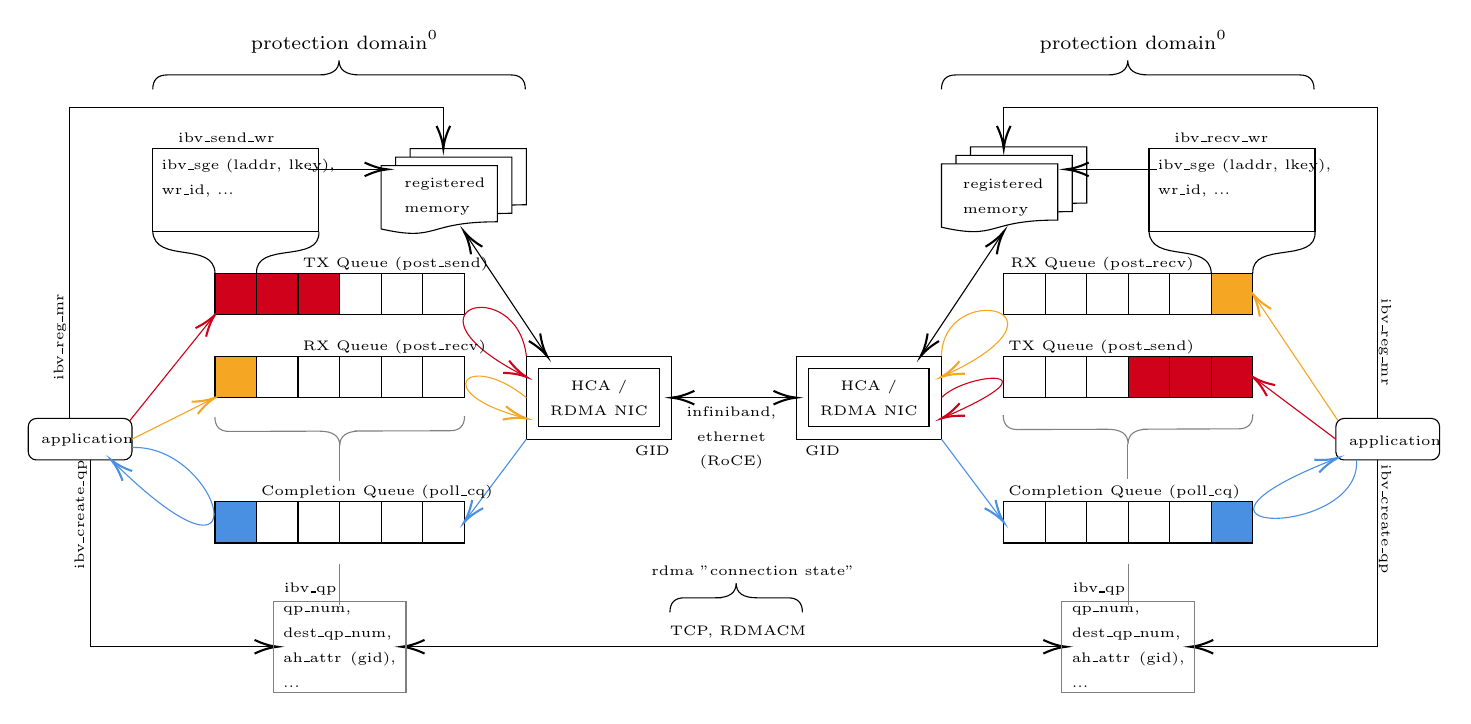
\begin{tikzpicture}[x=0.75pt,y=0.75pt,yscale=-1,xscale=1]
      \tikzset{every picture/.style={line width=0.75pt}} %set default line width to 0.75pt
%uncomment if require: \path (0,337); %set diagram left start at 0, and has height of 337

%Shape: Grid [id:dp4295659866532805]
\draw  [draw opacity=0] (100,220) -- (220,220) -- (220,240) -- (100,240) -- cycle ; \draw   (120,220) -- (120,240)(140,220) -- (140,240)(160,220) -- (160,240)(180,220) -- (180,240)(200,220) -- (200,240) ; \draw    ; \draw   (100,220) -- (220,220) -- (220,240) -- (100,240) -- cycle ;
%Shape: Grid [id:dp8946879606396433]
\draw  [draw opacity=0] (100,150) -- (220,150) -- (220,170) -- (100,170) -- cycle ; \draw   (120,150) -- (120,170)(140,150) -- (140,170)(160,150) -- (160,170)(180,150) -- (180,170)(200,150) -- (200,170) ; \draw    ; \draw   (100,150) -- (220,150) -- (220,170) -- (100,170) -- cycle ;
%Shape: Grid [id:dp4368011626744822]
\draw  [draw opacity=0] (100,110) -- (220,110) -- (220,130) -- (100,130) -- cycle ; \draw   (120,110) -- (120,130)(140,110) -- (140,130)(160,110) -- (160,130)(180,110) -- (180,130)(200,110) -- (200,130) ; \draw    ; \draw   (100,110) -- (220,110) -- (220,130) -- (100,130) -- cycle ;
%Shape: Frame [id:dp0617244658145758]
\draw   (250,150) -- (320,150) -- (320,190) -- (250,190) -- cycle(314,156) -- (256,156) -- (256,184) -- (314,184) -- cycle ;
%Curve Lines [id:da5967844605583035]
\draw [color={rgb, 255:red, 208; green, 2; blue, 27 }  ,draw opacity=1 ]   (250,150) .. controls (245.42,109.8) and (184.41,126.63) .. (249.02,159.5) ;
\draw [shift={(250,160)}, rotate = 206.63] [color={rgb, 255:red, 208; green, 2; blue, 27 }  ,draw opacity=1 ][line width=0.75]    (10.93,-3.29) .. controls (6.95,-1.4) and (3.31,-0.3) .. (0,0) .. controls (3.31,0.3) and (6.95,1.4) .. (10.93,3.29)   ;
%Straight Lines [id:da3545614732130127]
\draw [color={rgb, 255:red, 74; green, 144; blue, 226 }  ,draw opacity=1 ]   (250,190) -- (221.2,228.4) ;
\draw [shift={(220,230)}, rotate = 306.87] [color={rgb, 255:red, 74; green, 144; blue, 226 }  ,draw opacity=1 ][line width=0.75]    (10.93,-3.29) .. controls (6.95,-1.4) and (3.31,-0.3) .. (0,0) .. controls (3.31,0.3) and (6.95,1.4) .. (10.93,3.29)   ;
%Curve Lines [id:da204421881230066]
\draw [color={rgb, 255:red, 245; green, 166; blue, 35 }  ,draw opacity=1 ]   (250,170) .. controls (221.78,146.98) and (202.19,167.58) .. (248.57,179.64) ;
\draw [shift={(250,180)}, rotate = 193.98] [color={rgb, 255:red, 245; green, 166; blue, 35 }  ,draw opacity=1 ][line width=0.75]    (10.93,-3.29) .. controls (6.95,-1.4) and (3.31,-0.3) .. (0,0) .. controls (3.31,0.3) and (6.95,1.4) .. (10.93,3.29)   ;
%Shape: Rectangle [id:dp7444892557504112]
\draw   (70,50) -- (150,50) -- (150,90) -- (70,90) -- cycle ;
%Curve Lines [id:da4358799403511109]
\draw    (100,110) .. controls (99.4,94.4) and (71,105.6) .. (70,90) ;
%Curve Lines [id:da04054970173393413]
\draw    (120,110) .. controls (119.4,94.4) and (151,105.6) .. (150,90) ;
%Shape: Rectangle [id:dp09447409855918232]
\draw  [fill={rgb, 255:red, 208; green, 2; blue, 27 }  ,fill opacity=1 ] (140,110) -- (160,110) -- (160,130) -- (140,130) -- cycle ;
%Shape: Rectangle [id:dp7954961531438973]
\draw  [fill={rgb, 255:red, 208; green, 2; blue, 27 }  ,fill opacity=1 ] (120,110) -- (140,110) -- (140,130) -- (120,130) -- cycle ;
%Shape: Rectangle [id:dp375729093280755]
\draw  [fill={rgb, 255:red, 245; green, 166; blue, 35 }  ,fill opacity=1 ] (100,150) -- (120,150) -- (120,170) -- (100,170) -- cycle ;
%Shape: Rectangle [id:dp7009688837706805]
\draw  [fill={rgb, 255:red, 208; green, 2; blue, 27 }  ,fill opacity=1 ] (100,110) -- (120,110) -- (120,130) -- (100,130) -- cycle ;
%Shape: Rectangle [id:dp4753240489158659]
\draw  [fill={rgb, 255:red, 74; green, 144; blue, 226 }  ,fill opacity=1 ] (100,220) -- (120,220) -- (120,240) -- (100,240) -- cycle ;
%Rounded Rect [id:dp7482108927478565]
\draw   (10,184) .. controls (10,181.79) and (11.79,180) .. (14,180) -- (56,180) .. controls (58.21,180) and (60,181.79) .. (60,184) -- (60,196) .. controls (60,198.21) and (58.21,200) .. (56,200) -- (14,200) .. controls (11.79,200) and (10,198.21) .. (10,196) -- cycle ;
%Straight Lines [id:da0860623165459462]
\draw [color={rgb, 255:red, 208; green, 2; blue, 27 }  ,draw opacity=1 ]   (59,181) -- (98.75,131.56) ;
\draw [shift={(100,130)}, rotate = 488.8] [color={rgb, 255:red, 208; green, 2; blue, 27 }  ,draw opacity=1 ][line width=0.75]    (10.93,-3.29) .. controls (6.95,-1.4) and (3.31,-0.3) .. (0,0) .. controls (3.31,0.3) and (6.95,1.4) .. (10.93,3.29)   ;
%Straight Lines [id:da10819672911414313]
\draw [color={rgb, 255:red, 245; green, 166; blue, 35 }  ,draw opacity=1 ]   (60,190) -- (98.21,170.89) ;
\draw [shift={(100,170)}, rotate = 513.4300000000001] [color={rgb, 255:red, 245; green, 166; blue, 35 }  ,draw opacity=1 ][line width=0.75]    (10.93,-3.29) .. controls (6.95,-1.4) and (3.31,-0.3) .. (0,0) .. controls (3.31,0.3) and (6.95,1.4) .. (10.93,3.29)   ;
%Curve Lines [id:da5396028508269919]
\draw [color={rgb, 255:red, 74; green, 144; blue, 226 }  ,draw opacity=1 ]   (60,194) .. controls (102.79,192.41) and (125.18,273.98) .. (51.12,201.11) ;
\draw [shift={(50,200)}, rotate = 404.77] [color={rgb, 255:red, 74; green, 144; blue, 226 }  ,draw opacity=1 ][line width=0.75]    (10.93,-3.29) .. controls (6.95,-1.4) and (3.31,-0.3) .. (0,0) .. controls (3.31,0.3) and (6.95,1.4) .. (10.93,3.29)   ;
%Flowchart: Multidocument [id:dp5721236644573098]
\draw  [fill={rgb, 255:red, 255; green, 255; blue, 255 }  ,fill opacity=1 ] (194,50) -- (250,50) -- (250,77.06) .. controls (215,77.06) and (222,86.82) .. (194,80.5) -- cycle ; \draw  [fill={rgb, 255:red, 255; green, 255; blue, 255 }  ,fill opacity=1 ] (187,54.1) -- (243,54.1) -- (243,81.16) .. controls (208,81.16) and (215,90.92) .. (187,84.6) -- cycle ; \draw  [fill={rgb, 255:red, 255; green, 255; blue, 255 }  ,fill opacity=1 ] (180,58.2) -- (236,58.2) -- (236,85.26) .. controls (201,85.26) and (208,95.02) .. (180,88.7) -- cycle ;
%Straight Lines [id:da6912345896218269]
\draw    (145,60) -- (181,60) ;
\draw [shift={(183,60)}, rotate = 180] [color={rgb, 255:red, 0; green, 0; blue, 0 }  ][line width=0.75]    (10.93,-3.29) .. controls (6.95,-1.4) and (3.31,-0.3) .. (0,0) .. controls (3.31,0.3) and (6.95,1.4) .. (10.93,3.29)   ;
%Shape: Grid [id:dp119026641862925]
\draw  [draw opacity=0] (480,220) -- (600,220) -- (600,240) -- (480,240) -- cycle ; \draw   (500,220) -- (500,240)(520,220) -- (520,240)(540,220) -- (540,240)(560,220) -- (560,240)(580,220) -- (580,240) ; \draw    ; \draw   (480,220) -- (600,220) -- (600,240) -- (480,240) -- cycle ;
%Shape: Grid [id:dp0804991380561264]
\draw  [draw opacity=0] (480,150) -- (600,150) -- (600,170) -- (480,170) -- cycle ; \draw   (500,150) -- (500,170)(520,150) -- (520,170)(540,150) -- (540,170)(560,150) -- (560,170)(580,150) -- (580,170) ; \draw    ; \draw   (480,150) -- (600,150) -- (600,170) -- (480,170) -- cycle ;
%Shape: Grid [id:dp11715394785996025]
\draw  [draw opacity=0] (480,110) -- (600,110) -- (600,130) -- (480,130) -- cycle ; \draw   (500,110) -- (500,130)(520,110) -- (520,130)(540,110) -- (540,130)(560,110) -- (560,130)(580,110) -- (580,130) ; \draw    ; \draw   (480,110) -- (600,110) -- (600,130) -- (480,130) -- cycle ;
%Shape: Frame [id:dp8132523520793834]
\draw   (380,150) -- (450,150) -- (450,190) -- (380,190) -- cycle(444,156) -- (386,156) -- (386,184) -- (444,184) -- cycle ;
%Shape: Rectangle [id:dp9806953964426239]
\draw   (549.98,50) -- (629.98,50) -- (629.98,90) -- (549.98,90) -- cycle ;
%Curve Lines [id:da8538159727708337]
\draw    (579.98,110) .. controls (579.38,94.4) and (550.98,105.6) .. (549.98,90) ;
%Curve Lines [id:da503262725402064]
\draw    (599.98,110) .. controls (599.38,94.4) and (630.98,105.6) .. (629.98,90) ;
%Shape: Rectangle [id:dp23358801131092133]
\draw  [fill={rgb, 255:red, 208; green, 2; blue, 27 }  ,fill opacity=1 ] (580,150) -- (600,150) -- (600,170) -- (580,170) -- cycle ;
%Shape: Rectangle [id:dp16921311873779]
\draw  [fill={rgb, 255:red, 208; green, 2; blue, 27 }  ,fill opacity=1 ] (560,150) -- (580,150) -- (580,170) -- (560,170) -- cycle ;
%Shape: Rectangle [id:dp1685110147344583]
\draw  [fill={rgb, 255:red, 245; green, 166; blue, 35 }  ,fill opacity=1 ] (580,110) -- (600,110) -- (600,130) -- (580,130) -- cycle ;
%Shape: Rectangle [id:dp5932409601304787]
\draw  [fill={rgb, 255:red, 208; green, 2; blue, 27 }  ,fill opacity=1 ] (540,150) -- (560,150) -- (560,170) -- (540,170) -- cycle ;
%Shape: Rectangle [id:dp5864080847756401]
\draw  [fill={rgb, 255:red, 74; green, 144; blue, 226 }  ,fill opacity=1 ] (580,220) -- (600,220) -- (600,240) -- (580,240) -- cycle ;
%Rounded Rect [id:dp9740510619526319]
\draw   (640,184) .. controls (640,181.79) and (641.79,180) .. (644,180) -- (686,180) .. controls (688.21,180) and (690,181.79) .. (690,184) -- (690,196) .. controls (690,198.21) and (688.21,200) .. (686,200) -- (644,200) .. controls (641.79,200) and (640,198.21) .. (640,196) -- cycle ;
%Straight Lines [id:da16241601875679856]
\draw [color={rgb, 255:red, 208; green, 2; blue, 27 }  ,draw opacity=1 ]   (640,190) -- (601.6,161.2) ;
\draw [shift={(600,160)}, rotate = 396.87] [color={rgb, 255:red, 208; green, 2; blue, 27 }  ,draw opacity=1 ][line width=0.75]    (10.93,-3.29) .. controls (6.95,-1.4) and (3.31,-0.3) .. (0,0) .. controls (3.31,0.3) and (6.95,1.4) .. (10.93,3.29)   ;
%Straight Lines [id:da918563124412445]
\draw [color={rgb, 255:red, 245; green, 166; blue, 35 }  ,draw opacity=1 ]   (641,181) -- (601.12,121.66) ;
\draw [shift={(600,120)}, rotate = 416.09000000000003] [color={rgb, 255:red, 245; green, 166; blue, 35 }  ,draw opacity=1 ][line width=0.75]    (10.93,-3.29) .. controls (6.95,-1.4) and (3.31,-0.3) .. (0,0) .. controls (3.31,0.3) and (6.95,1.4) .. (10.93,3.29)   ;
%Curve Lines [id:da07688196394851687]
\draw [color={rgb, 255:red, 74; green, 144; blue, 226 }  ,draw opacity=1 ]   (650,200) .. controls (652.32,238.47) and (544.75,236.69) .. (639.56,199.56) ;
\draw [shift={(641,199)}, rotate = 518.8399999999999] [color={rgb, 255:red, 74; green, 144; blue, 226 }  ,draw opacity=1 ][line width=0.75]    (10.93,-3.29) .. controls (6.95,-1.4) and (3.31,-0.3) .. (0,0) .. controls (3.31,0.3) and (6.95,1.4) .. (10.93,3.29)   ;
%Flowchart: Multidocument [id:dp24323844239769876]
\draw  [fill={rgb, 255:red, 255; green, 255; blue, 255 }  ,fill opacity=1 ] (464,49.17) -- (520,49.17) -- (520,76.23) .. controls (485,76.23) and (492,85.99) .. (464,79.67) -- cycle ; \draw  [fill={rgb, 255:red, 255; green, 255; blue, 255 }  ,fill opacity=1 ] (457,53.27) -- (513,53.27) -- (513,80.33) .. controls (478,80.33) and (485,90.09) .. (457,83.77) -- cycle ; \draw  [fill={rgb, 255:red, 255; green, 255; blue, 255 }  ,fill opacity=1 ] (450,57.37) -- (506,57.37) -- (506,84.43) .. controls (471,84.43) and (478,94.19) .. (450,87.87) -- cycle ;
%Straight Lines [id:da7059822979397073]
\draw    (660,180) -- (660,30) ;
%Straight Lines [id:da481201579183531]
\draw    (512,60) -- (554,60) ;
\draw [shift={(510,60)}, rotate = 0] [color={rgb, 255:red, 0; green, 0; blue, 0 }  ][line width=0.75]    (10.93,-3.29) .. controls (6.95,-1.4) and (3.31,-0.3) .. (0,0) .. controls (3.31,0.3) and (6.95,1.4) .. (10.93,3.29)   ;
%Straight Lines [id:da22589634957435445]
\draw [color={rgb, 255:red, 0; green, 0; blue, 0 }  ,draw opacity=1 ]   (322,170) -- (378,170) ;
\draw [shift={(380,170)}, rotate = 180] [color={rgb, 255:red, 0; green, 0; blue, 0 }  ,draw opacity=1 ][line width=0.75]    (10.93,-3.29) .. controls (6.95,-1.4) and (3.31,-0.3) .. (0,0) .. controls (3.31,0.3) and (6.95,1.4) .. (10.93,3.29)   ;
\draw [shift={(320,170)}, rotate = 0] [color={rgb, 255:red, 0; green, 0; blue, 0 }  ,draw opacity=1 ][line width=0.75]    (10.93,-3.29) .. controls (6.95,-1.4) and (3.31,-0.3) .. (0,0) .. controls (3.31,0.3) and (6.95,1.4) .. (10.93,3.29)   ;
%Straight Lines [id:da11720587390108372]
\draw    (192,290) -- (508,290) ;
\draw [shift={(510,290)}, rotate = 180] [color={rgb, 255:red, 0; green, 0; blue, 0 }  ][line width=0.75]    (10.93,-3.29) .. controls (6.95,-1.4) and (3.31,-0.3) .. (0,0) .. controls (3.31,0.3) and (6.95,1.4) .. (10.93,3.29)   ;
\draw [shift={(190,290)}, rotate = 0] [color={rgb, 255:red, 0; green, 0; blue, 0 }  ][line width=0.75]    (10.93,-3.29) .. controls (6.95,-1.4) and (3.31,-0.3) .. (0,0) .. controls (3.31,0.3) and (6.95,1.4) .. (10.93,3.29)   ;
%Curve Lines [id:da21032506501189785]
\draw [color={rgb, 255:red, 245; green, 166; blue, 35 }  ,draw opacity=1 ]   (450,150) .. controls (450.6,112.59) and (520.69,127.45) .. (451.06,159.52) ;
\draw [shift={(450,160)}, rotate = 335.59000000000003] [color={rgb, 255:red, 245; green, 166; blue, 35 }  ,draw opacity=1 ][line width=0.75]    (10.93,-3.29) .. controls (6.95,-1.4) and (3.31,-0.3) .. (0,0) .. controls (3.31,0.3) and (6.95,1.4) .. (10.93,3.29)   ;
%Curve Lines [id:da1795237296648432]
\draw [color={rgb, 255:red, 208; green, 2; blue, 27 }  ,draw opacity=1 ]   (450,170) .. controls (461.68,157.72) and (508.84,154.46) .. (451.76,179.24) ;
\draw [shift={(450,180)}, rotate = 336.82] [color={rgb, 255:red, 208; green, 2; blue, 27 }  ,draw opacity=1 ][line width=0.75]    (10.93,-3.29) .. controls (6.95,-1.4) and (3.31,-0.3) .. (0,0) .. controls (3.31,0.3) and (6.95,1.4) .. (10.93,3.29)   ;
%Straight Lines [id:da2007010103317477]
\draw [color={rgb, 255:red, 74; green, 144; blue, 226 }  ,draw opacity=1 ]   (450,190) -- (478.8,228.4) ;
\draw [shift={(480,230)}, rotate = 233.13] [color={rgb, 255:red, 74; green, 144; blue, 226 }  ,draw opacity=1 ][line width=0.75]    (10.93,-3.29) .. controls (6.95,-1.4) and (3.31,-0.3) .. (0,0) .. controls (3.31,0.3) and (6.95,1.4) .. (10.93,3.29)   ;
%Shape: Brace [id:dp9940577590245101]
\draw   (383,273.42) .. controls (383,268.75) and (380.67,266.42) .. (376,266.42) -- (361.08,266.42) .. controls (354.41,266.42) and (351.08,264.09) .. (351.08,259.42) .. controls (351.08,264.09) and (347.75,266.42) .. (341.08,266.42)(344.08,266.42) -- (326.17,266.42) .. controls (321.5,266.42) and (319.17,268.75) .. (319.17,273.42) ;
%Straight Lines [id:da4361920428251189]
\draw    (660,200) -- (660,290) ;
%Straight Lines [id:da480314407062288]
\draw    (40,200) -- (40,290) ;
%Shape: Brace [id:dp588298908527398]
\draw  [color={rgb, 255:red, 128; green, 128; blue, 128 }  ,draw opacity=1 ] (99.93,179.28) .. controls (99.95,183.95) and (102.29,186.27) .. (106.96,186.26) -- (150.09,186.13) .. controls (156.76,186.1) and (160.1,188.42) .. (160.11,193.09) .. controls (160.1,188.42) and (163.42,186.08) .. (170.09,186.06)(167.09,186.07) -- (213.22,185.93) .. controls (217.89,185.92) and (220.21,183.58) .. (220.2,178.91) ;
%Straight Lines [id:da0889380362629657]
\draw    (40,290) -- (128,290) ;
\draw [shift={(130,290)}, rotate = 180] [color={rgb, 255:red, 0; green, 0; blue, 0 }  ][line width=0.75]    (10.93,-3.29) .. controls (6.95,-1.4) and (3.31,-0.3) .. (0,0) .. controls (3.31,0.3) and (6.95,1.4) .. (10.93,3.29)   ;
%Straight Lines [id:da17063350648323872]
\draw [color={rgb, 255:red, 128; green, 128; blue, 128 }  ,draw opacity=1 ]   (160,193) -- (160,210) ;
%Straight Lines [id:da735591769614332]
\draw [color={rgb, 255:red, 128; green, 128; blue, 128 }  ,draw opacity=1 ]   (160,250) -- (160,270) ;
%Shape: Brace [id:dp7463787220884971]
\draw  [color={rgb, 255:red, 128; green, 128; blue, 128 }  ,draw opacity=1 ] (479.73,178.38) .. controls (479.75,183.05) and (482.09,185.37) .. (486.76,185.36) -- (529.89,185.22) .. controls (536.56,185.2) and (539.9,187.52) .. (539.91,192.19) .. controls (539.9,187.52) and (543.22,185.18) .. (549.89,185.16)(546.89,185.17) -- (593.02,185.02) .. controls (597.69,185.01) and (600.01,182.67) .. (600,178) ;
%Straight Lines [id:da6347067855883498]
\draw [color={rgb, 255:red, 128; green, 128; blue, 128 }  ,draw opacity=1 ]   (539.8,192.09) -- (539.8,209.09) ;
%Straight Lines [id:da7879312663238379]
\draw [color={rgb, 255:red, 128; green, 128; blue, 128 }  ,draw opacity=1 ]   (540,250) -- (540,270) ;
%Straight Lines [id:da34735570105619973]
\draw    (660,290) -- (572,290) ;
\draw [shift={(570,290)}, rotate = 360] [color={rgb, 255:red, 0; green, 0; blue, 0 }  ][line width=0.75]    (10.93,-3.29) .. controls (6.95,-1.4) and (3.31,-0.3) .. (0,0) .. controls (3.31,0.3) and (6.95,1.4) .. (10.93,3.29)   ;
%Straight Lines [id:da6922947722733842]
\draw    (480,30) -- (660,30) ;
%Straight Lines [id:da8214317936198106]
\draw    (480,30) -- (480,48) ;
\draw [shift={(480,50)}, rotate = 270] [color={rgb, 255:red, 0; green, 0; blue, 0 }  ][line width=0.75]    (10.93,-3.29) .. controls (6.95,-1.4) and (3.31,-0.3) .. (0,0) .. controls (3.31,0.3) and (6.95,1.4) .. (10.93,3.29)   ;
%Straight Lines [id:da3127224438135543]
\draw    (30,180) -- (30,30) ;
%Straight Lines [id:da25223149816814294]
\draw    (30,30) -- (210,30) ;
%Straight Lines [id:da6150923577431217]
\draw    (210,30) -- (210,48) ;
\draw [shift={(210,50)}, rotate = 270] [color={rgb, 255:red, 0; green, 0; blue, 0 }  ][line width=0.75]    (10.93,-3.29) .. controls (6.95,-1.4) and (3.31,-0.3) .. (0,0) .. controls (3.31,0.3) and (6.95,1.4) .. (10.93,3.29)   ;
%Shape: Brace [id:dp7460733200764286]
\draw   (249.5,21.5) .. controls (249.5,16.83) and (247.17,14.5) .. (242.5,14.5) -- (169.75,14.5) .. controls (163.08,14.5) and (159.75,12.17) .. (159.75,7.5) .. controls (159.75,12.17) and (156.42,14.5) .. (149.75,14.5)(152.75,14.5) -- (77,14.5) .. controls (72.33,14.5) and (70,16.83) .. (70,21.5) ;
%Shape: Brace [id:dp25327117875899263]
\draw   (629.5,21.5) .. controls (629.5,16.83) and (627.17,14.5) .. (622.5,14.5) -- (549.75,14.5) .. controls (543.08,14.5) and (539.75,12.17) .. (539.75,7.5) .. controls (539.75,12.17) and (536.42,14.5) .. (529.75,14.5)(532.75,14.5) -- (457,14.5) .. controls (452.33,14.5) and (450,16.83) .. (450,21.5) ;
%Straight Lines [id:da5693657957631059]
\draw    (221.11,91.66) -- (258.89,148.34) ;
\draw [shift={(260,150)}, rotate = 236.31] [color={rgb, 255:red, 0; green, 0; blue, 0 }  ][line width=0.75]    (10.93,-3.29) .. controls (6.95,-1.4) and (3.31,-0.3) .. (0,0) .. controls (3.31,0.3) and (6.95,1.4) .. (10.93,3.29)   ;
\draw [shift={(220,90)}, rotate = 56.31] [color={rgb, 255:red, 0; green, 0; blue, 0 }  ][line width=0.75]    (10.93,-3.29) .. controls (6.95,-1.4) and (3.31,-0.3) .. (0,0) .. controls (3.31,0.3) and (6.95,1.4) .. (10.93,3.29)   ;
%Straight Lines [id:da648148726214795]
\draw    (478.89,91.66) -- (441.11,148.34) ;
\draw [shift={(440,150)}, rotate = 303.69] [color={rgb, 255:red, 0; green, 0; blue, 0 }  ][line width=0.75]    (10.93,-3.29) .. controls (6.95,-1.4) and (3.31,-0.3) .. (0,0) .. controls (3.31,0.3) and (6.95,1.4) .. (10.93,3.29)   ;
\draw [shift={(480,90)}, rotate = 123.69] [color={rgb, 255:red, 0; green, 0; blue, 0 }  ][line width=0.75]    (10.93,-3.29) .. controls (6.95,-1.4) and (3.31,-0.3) .. (0,0) .. controls (3.31,0.3) and (6.95,1.4) .. (10.93,3.29)   ;

% Text Node
\draw (121,211) node [anchor=north west][inner sep=0.75pt]  [font=\tiny] [align=left] {Completion Queue (poll\_cq)};
% Text Node
\draw (141,101) node [anchor=north west][inner sep=0.75pt]  [font=\tiny] [align=left] {TX Queue (post\_send)};
% Text Node
\draw (141,141) node [anchor=north west][inner sep=0.75pt]  [font=\tiny] [align=left] {RX Queue (post\_recv)};
% Text Node
\draw (81,41) node [anchor=north west][inner sep=0.75pt]  [font=\tiny] [align=left] {ibv\_send\_wr};
% Text Node
\draw (73,54) node [anchor=north west][inner sep=0.75pt]  [font=\tiny] [align=left] {ibv\_sge (laddr, lkey),\\wr\_id, ...};
% Text Node
\draw (15,186) node [anchor=north west][inner sep=0.75pt]  [font=\tiny] [align=left] {application};
% Text Node
\draw (190,63) node [anchor=north west][inner sep=0.75pt]  [font=\tiny] [align=left] {registered\\memory};
% Text Node
\draw (21,163) node [anchor=north west][inner sep=0.75pt]  [font=\tiny,rotate=-270] [align=left] {ibv\_reg\_mr};
% Text Node
\draw (481,141) node [anchor=north west][inner sep=0.75pt]  [font=\tiny] [align=left] {TX Queue (post\_send)};
% Text Node
\draw (482,101) node [anchor=north west][inner sep=0.75pt]  [font=\tiny] [align=left] {RX Queue (post\_recv)};
% Text Node
\draw (560.98,41) node [anchor=north west][inner sep=0.75pt]  [font=\tiny] [align=left] {ibv\_recv\_wr};
% Text Node
\draw (552.98,54) node [anchor=north west][inner sep=0.75pt]  [font=\tiny] [align=left] {ibv\_sge (laddr, lkey),\\wr\_id, ...};
% Text Node
\draw (645,187) node [anchor=north west][inner sep=0.75pt]  [font=\tiny] [align=left] {application};
% Text Node
\draw (459,63.17) node [anchor=north west][inner sep=0.75pt]  [font=\tiny] [align=left] {registered\\memory};
% Text Node
\draw (668,121) node [anchor=north west][inner sep=0.75pt]  [font=\tiny,rotate=-90] [align=left] {ibv\_reg\_mr};
% Text Node
\draw (321,173) node [anchor=north west][inner sep=0.75pt]  [font=\tiny] [align=left] {\begin{minipage}[lt]{39.83664400000001pt}\setlength\topsep{0pt}
\begin{center}
infiniband,\\ethernet (RoCE)
\end{center}

\end{minipage}};
% Text Node
\draw (481,211) node [anchor=north west][inner sep=0.75pt]  [font=\tiny] [align=left] {Completion Queue (poll\_cq)};
% Text Node
\draw (285,170) node  [font=\tiny] [align=left] {\begin{minipage}[lt]{39.440000000000005pt}\setlength\topsep{0pt}
\begin{center}
HCA /\\RDMA NIC
\end{center}

\end{minipage}};
% Text Node
\draw (415,170) node  [font=\tiny] [align=left] {\begin{minipage}[lt]{39.440000000000005pt}\setlength\topsep{0pt}
\begin{center}
HCA /\\RDMA NIC
\end{center}

\end{minipage}};
% Text Node
\draw (301,192) node [anchor=north west][inner sep=0.75pt]  [font=\tiny] [align=left] {GID};
% Text Node
\draw (383,192) node [anchor=north west][inner sep=0.75pt]  [font=\tiny] [align=left] {GID};
% Text Node
\draw  [color={rgb, 255:red, 128; green, 128; blue, 128 }  ,draw opacity=1 ]  (128,268) -- (192,268) -- (192,312) -- (128,312) -- cycle  ;
\draw (160,290) node  [font=\tiny] [align=left] {\begin{minipage}[lt]{40.800000000000004pt}\setlength\topsep{0pt}
qp\_num, dest\_qp\_num, ah\_attr (gid), ...
\end{minipage}};
% Text Node
\draw (132,258) node [anchor=north west][inner sep=0.75pt]  [font=\tiny] [align=left] {ibv\_qp};
% Text Node
\draw (309,250) node [anchor=north west][inner sep=0.75pt]  [font=\tiny] [align=left] {rdma "connection state"};
% Text Node
\draw (31,254) node [anchor=north west][inner sep=0.75pt]  [font=\tiny,rotate=-270] [align=left] {ibv\_create\_qp};
% Text Node
\draw (668,201) node [anchor=north west][inner sep=0.75pt]  [font=\tiny,rotate=-90] [align=left] {ibv\_create\_qp};
% Text Node
\draw (352,283) node  [font=\tiny] [align=left] {\begin{minipage}[lt]{68pt}\setlength\topsep{0pt}
\begin{center}
TCP, RDMACM
\end{center}

\end{minipage}};
% Text Node
\draw  [color={rgb, 255:red, 128; green, 128; blue, 128 }  ,draw opacity=1 ]  (508,268) -- (572,268) -- (572,312) -- (508,312) -- cycle  ;
\draw (540,290) node  [font=\tiny] [align=left] {\begin{minipage}[lt]{40.800000000000004pt}\setlength\topsep{0pt}
qp\_num, dest\_qp\_num, ah\_attr (gid), ...
\end{minipage}};
% Text Node
\draw (512,258) node [anchor=north west][inner sep=0.75pt]  [font=\tiny] [align=left] {ibv\_qp};
% Text Node
\draw (116,-8) node [anchor=north west][inner sep=0.75pt]  [font=\scriptsize] [align=left] {protection domain$\displaystyle ^{0}$};
% Text Node
\draw (496,-8) node [anchor=north west][inner sep=0.75pt]  [font=\scriptsize] [align=left] {protection domain$\displaystyle ^{0}$};

   \end{tikzpicture}
}
\end{document}
